\section{Results}
\label{results}

We start by describing the results for each study in detail, before proceeding to summarize and discuss the observed effects.

\subsection{Experimental Simulation}
\label{sec:expResults}

In Table~\ref{tab:results} we summarize the results from the 24 trials. Those participants mixed graduates working in industry (41.6\%) and graduates during their M.Sc. and Ph.D. studies (58.4\%).



\begin{table}
\centering
\caption{Experimental results, for each treatment (textual Javadoc \emph{JavaDoc}, \contractjdoc{} \emph{ContJDoc} and formal contracts \emph{Formal}. For each API (Queue or Stack) and Task (\emph{Cli} if a client for the API was implemented, \emph{Sup} if an implementation for the API was provided), participants are listed (\emph{Part}) along with the result (\emph{Res}) from our test cases.}
\label{tab:results}
\begin{tabular}{|l|l||l|l||l|l||l|l|} 
\cline{3-8}
\multicolumn{1}{l}{} &              & \multicolumn{2}{l||}{\textbf{JavaDoc }} & \multicolumn{2}{l||}{\textbf{ContJDoc }} & \multicolumn{2}{l|}{\textbf{Formal}}  \\ 
\hline
\uline{DataStr}      & \uline{Task} & Part & Res                              & Part & Res                                & Part & Res                             \\ 
\hline\hline
\uline{Queue}        & \uline{Cli}  & p9   & \greencheck       & p11  & \redcross                                    & p7   & \greencheck                                 \\
                     & \uline{Cli}  & p10  & \greencheck                                 & p12  & \redcross                                    & p8   & \redcross                                \\
                     & \uline{Sup}  & p21  & \greencheck                                 & p23  & \greencheck                                    & p19  &  \greencheck                               \\
                     & \uline{Sup}  & p22  & \redcross                                 & p24  & \greencheck                                    & p20  &  \redcross                               \\ 
\hline\hline
\uline{Stack}        & \uline{Cli}  & p3   & \redcross                                 & p5   & \redcross                                    & p1   & \redcross                                 \\
                     & \uline{Cli}  & p4   & \redcross                                 & p6   & \redcross                                    & p2   & \greencheck                                 \\
                     & \uline{Sup}  & p15  & \greencheck                                 & p17  & \redcross                                    & p13  & \redcross                                \\
                     & \uline{Sup}  & p16  & \greencheck                                 & p18  & \greencheck                                    & p14  & \redcross                                \\
\hline
\end{tabular}
\end{table}



Table~\ref{tab:faults} details the faults that were found in the participants' code.

\begin{table}
\centering
\caption{Reason (fault) for failures in participants' results}
\label{tab:faults}
\begin{adjustbox}{width=\textwidth}
\begin{tabular}{|l|l|l|l|} 
\hline
\multicolumn{4}{|l|}{\textbf{Javadoc} }                                                                                                                                                                         \\ 
\hline
p22                                        & Queue                             & Sup                                & Code error (method \textbackslash{}texttt\{add\})                                         \\ 
\hline
p3                                         & Stack                             & Cli                                & Contract Failure (invariant on all methods)                                               \\ 
\hline
p4                                         & Stack                             & Cli                                & Contract Failure (does not fulfil several post-conditions)                                \\ 
\hline
\multicolumn{4}{|l|}{\textbf{ContractJDoc }}                                                                                                                                                                    \\ 
\hline
p11                                        & Queue                             & Cli                                & Unfinished task                                                                           \\ 
\hline
p12                                        & Queue                             & Cli                                & Unfinished task                                                                           \\ 
\hline
p5                                         & Stack                             & Cli                                & Contract Failure (pre-condition on method \textbackslash{}texttt\{consumeService\})       \\ 
\hline
p6                                         & Stack                             & Cli                                & Code error (internal manipulation)                                                        \\ 
\hline
p17                                        & Stack                             & Sup                                & Contract Failure (invariant unfulfilled in the stack)                                     \\ 
\hline
\multicolumn{4}{|l|}{\textbf{Formal contracts} }                                                                                                                                                                \\ 
\hline
p8                                         & Queue                             & Cli                                & Contract Failure (invariant on all methods)                                               \\ 
\hline
p1                                         & Stack                             & Sup                                & Contract Failure (post-condition on method \textbackslash{}texttt\{removeAccountTop\})    \\ 
\hline
p13                                        & Stack                             & Sup                                & Contract Failure (post-condition unfulfilled on method \textbackslash{}texttt\{pop\})     \\ 
\hline
p14                                        & Stack                             & Sup                                & Contract Failure (post-condition unfulfilled on method \textbackslash{}texttt\{pop\})     \\ 
\hline
p20                                        & Queue                             & Sup                                & Contract Failure (post-condition unfulfilled on method \textbackslash{}texttt\{remove\})  \\ 
\hline\hline
\multicolumn{1}{|c|}{\textbf{Part}} & \multicolumn{1}{c|}{\textbf{API}} & \multicolumn{1}{c|}{\textbf{Task}} & \multicolumn{1}{c|}{\textbf{Type of~Fault}}                                               \\
\hline
\end{tabular}
\end{adjustbox}
\end{table}






% difficulty
Concerning the task performed by the developers, we present in
Figure \ref{fig:tasksEmpirical}
answers on difficulty grouped by the task performed.
The implementation of the documented interface (Supplier task) seemed to be easier
than the task of creating a Client class, however, this difference is not
statistically significant as presented by a Wilcoxon rank sum test~\cite{statistical}
(p-value = 0.07, confidence level of 95\%).
%

\begin{figure*}
\centering
\begin{subfigure}{.3\textwidth}
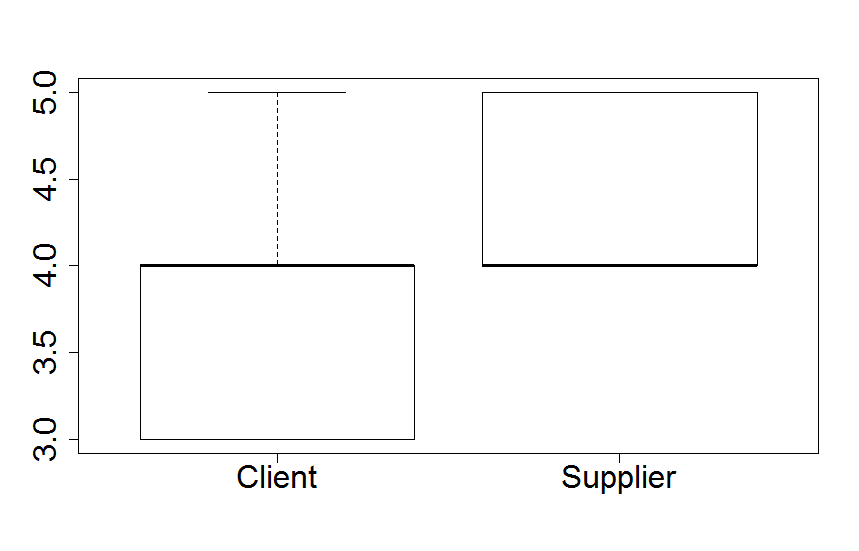
\includegraphics[width=1\linewidth]{figs/boxplotTasksEmpiricalStudy}
\caption{}
\label{fig:tasksEmpirical}
\end{subfigure}
\begin{subfigure}{.3\textwidth}
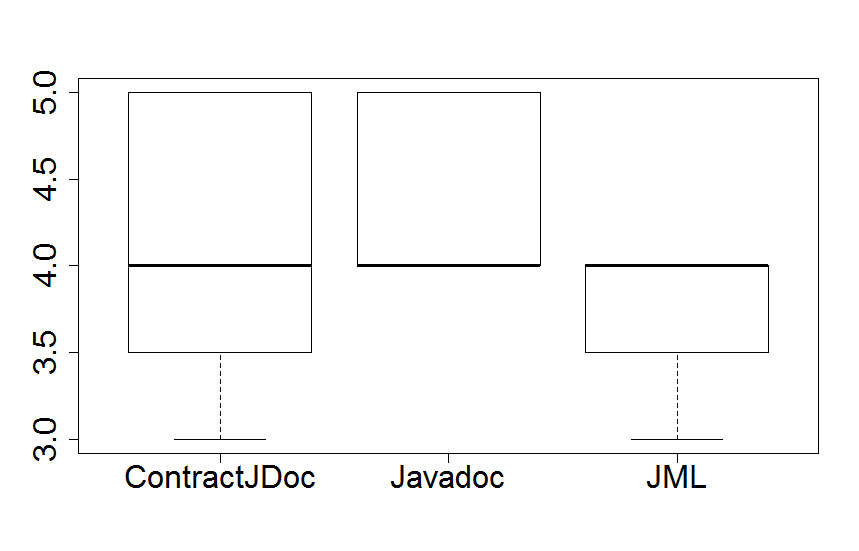
\includegraphics[width=1\linewidth]{figs/boxplotApproachesEmpiricalStudy}
\caption{}
\label{fig:approachesEmpirical}
\end{subfigure}
\begin{subfigure}{.3\textwidth}
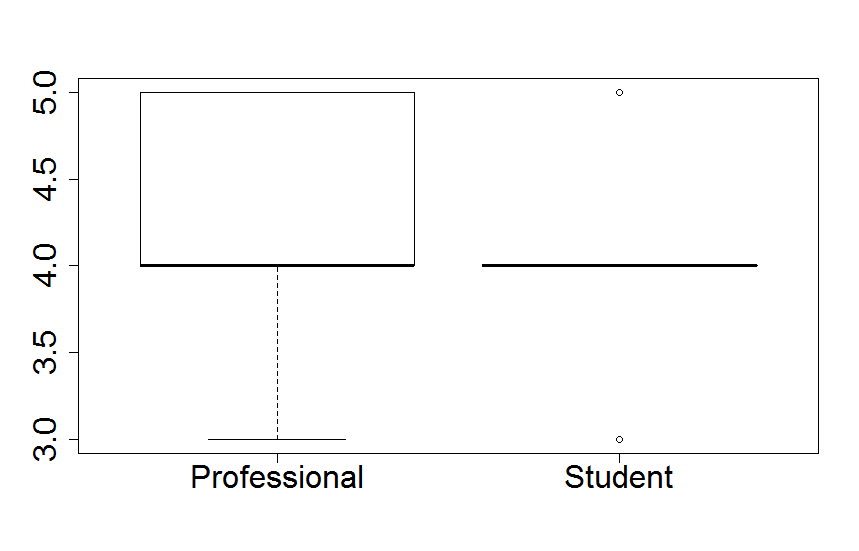
\includegraphics[width=1\linewidth]{figs/boxplotExperienceEmpiricalStudy}
\caption{}
\label{fig:experienceEmpirical}
\end{subfigure}
\caption{Results of our empirical study with Java developers, on an implementation task based on a
documented-interface, aiming to evaluate the readability and understandability of three approaches
for documenting Java code.}
\label{fig:empiricalResults}
\end{figure*}


% \begin{figure}
% \centering
% 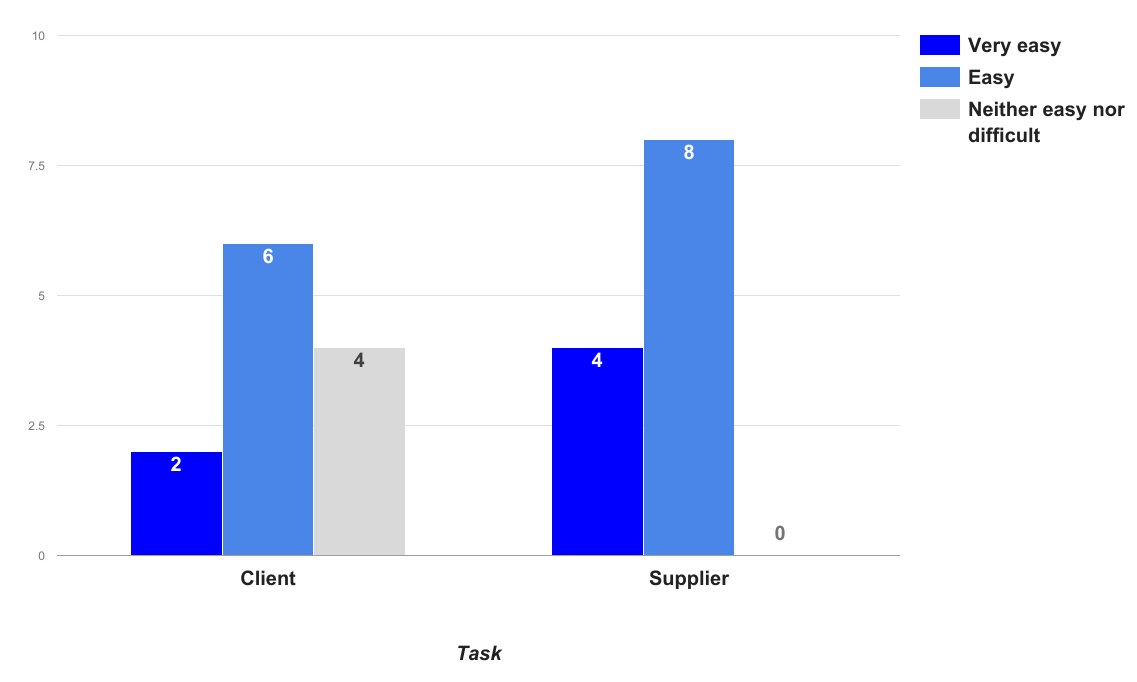
\includegraphics[width=1.0\textwidth]{figs/TaskComplexity}
% \caption{Answers grouped by task complexity.}
% \label{fig:taskComplexity}
% \end{figure}

% documenting approach
When grouped by documenting approach (see Figure \ref{fig:approachesEmpirical}),
the Kruskal-Wallis rank sum test showed no difference between the approaches
(p-value = 0.15).

% , the results present Javadoc as the easiest approach to be understood (see Figures \ref{fig:empiricalResults}(c),
% \ref{fig:empiricalResults}(d), and \ref{fig:empiricalResults}(e)). This is
% expected since Javadoc is a well established approach for documenting Java code. In addition, \contractjdoc{} was perceived as easier than JML: there are three answers \textit{Very easy} for \contractjdoc{} whereas
% there is no answer \textit{Very easy} for JML.

% experience
When grouped by experience (Figure \ref{fig:experienceEmpirical}), the Wilcoxon
rank sum test (p-value = 0.45) also does not show differences statistically
significant between professionals and students. 

% source code correct
Javadoc and \contractjdoc{} were the only documenting approaches in
which all participants were able to produce a code satisfying the oracle
(respecting the restrictions available in the comments). On the other hand,
there was one case developed by following the JML documenting approach in which
the contract is not satisfied by the implementation.





\subsection{Judgment Survey}
\label{sec:surveyResults}

142 Java developers answered the survey.
From those, 
51 are professionals (36\%) and 91 are students
(64\%).

%results - in general
With respect to the survey answers, 50.7\% (72) of the Subjects chose Javadoc as
the simplest approach to understand when using it in a general context. In addition,
for 38\% (54) of the subjects Javadoc is also the most understandable approach
with regard to the provided interface.

\begin{figure*}
\centering
\begin{subfigure}{.48\textwidth}
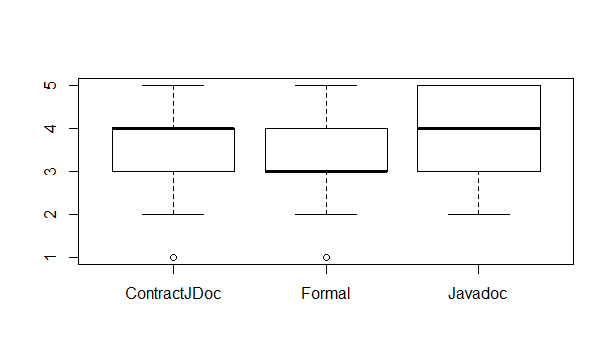
\includegraphics[width=1\linewidth]{figs/boxplotApproachesSurveyStudy}
\caption{All approaches}
\label{fig:allApproaches}
\end{subfigure}
\begin{subfigure}{.48\textwidth}
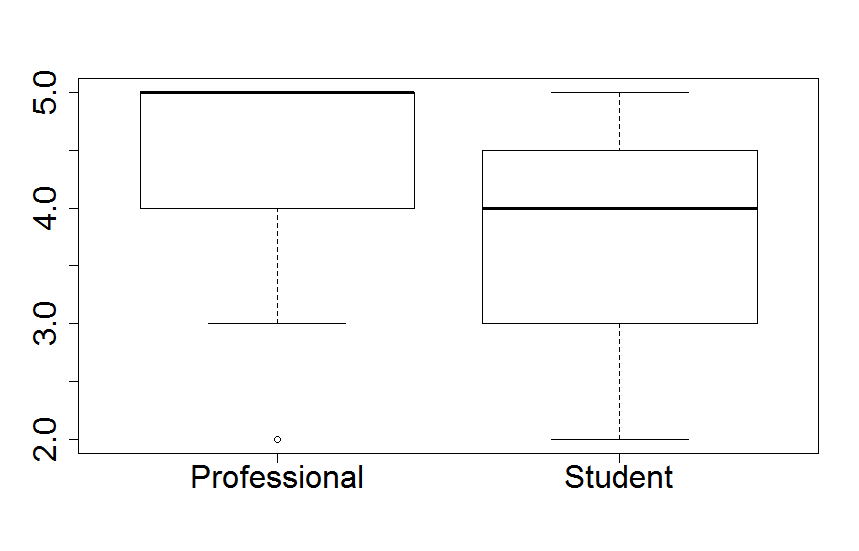
\includegraphics[width=1\linewidth]{figs/boxPlotJavadocXExperience}
\caption{Javadoc}
\label{fig:javadocExp}
\end{subfigure}
\\[1ex]
\begin{subfigure}{.48\textwidth}
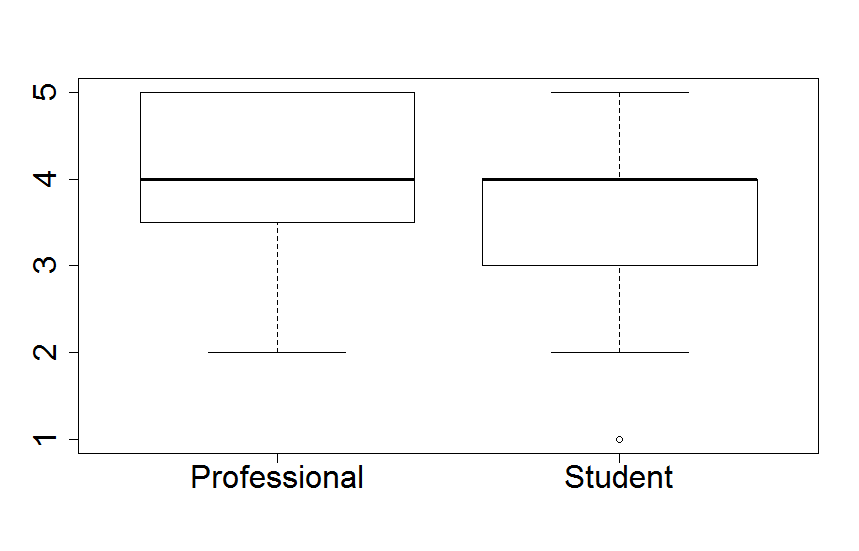
\includegraphics[width=1\linewidth]{figs/boxplotContractJDocXExperience.png}
\caption{\contractjdoc{}}
\label{fig:contractjdocExp}
\end{subfigure}
\begin{subfigure}{.48\textwidth}
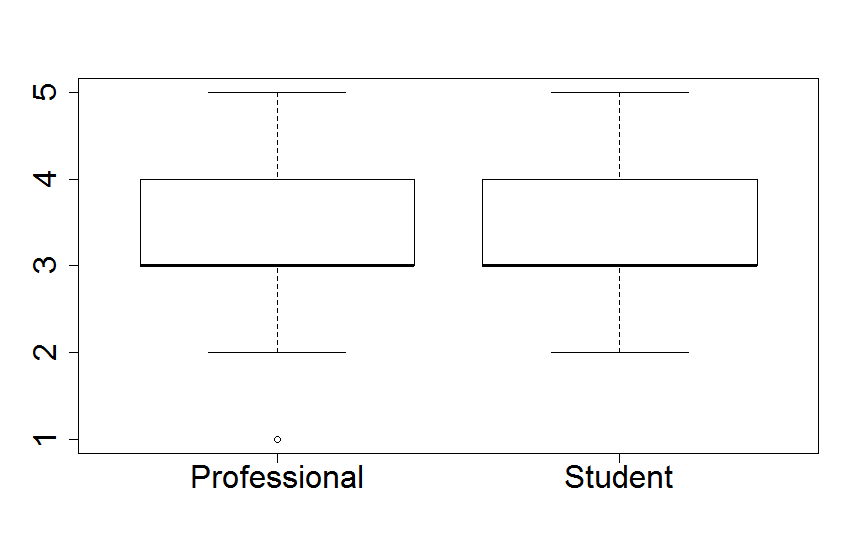
\includegraphics[width=1\linewidth]{figs/boxplotJMLXExperience.png}
\caption{JML}
\label{fig:jmlExp}
\end{subfigure}
\caption{Subjects' answers to the individual evaluation of comprehensibility for
each documentation approach. And answers grouped by experience for each
approach.}
\label{fig:surveyResults}
\end{figure*}

% continues
The survey results provided us statistical difference when comparing the the
comprehensibility of the documentation approaches evaluated (see
Figure~\ref{fig:allApproaches}). By performing an Oneway ANOVA test~\cite{statistical} and
a corresponding post hoc analysis we were able to distinguish the three
approaches (p-value $<$ 0.05).
The Tukey HSD~\cite{statistical} and pairwise comparisons using t tests
with Bonferroni correction~\cite{statistical} produced the following p-values:
Javadoc-ContractJDoc = 0.012, JML-ContractJDoc = 0.000, and JML-Javadoc = 0.000.

When analyzing data grouped by experience (Figures~\ref{fig:javadocExp} to
~\ref{fig:jmlExp}) by means of Wilcoxon rank sum test with continuity correction
tests, only for JML we found no statistical difference between Professionals and
Students (p-value = 0.17). For both Javadoc and \contractjdoc{}, Professionals
had perceived the approaches as being easier for comprehensing than Students
(p-value = 0.012 and p-value = 0.004, respectively).


\subsubsection{Comprehensibility Survey}
\label{sec:surveyDiscussion}





\subsection{Case Study}

Table~\ref{tab:caseStudyResults} presents the results of applying \contractjdoc{} to each system.
Column \#Clauses displays the number of clauses manually added in each system.
Column \#Errors presents the number of errors detected by the systems test suite after compiling the source code enhanced with contracts in
\contractjdoc{} approach. Column Time reveals the time (in seconds) needed for compiling the whole
project with its dependencies after applying \contractjdoc{} contracts. Columns \#Com.Case to \#Repet.
show the contract clauses added in each system grouped by type (following the
definitions from ~\cite{typeContracts}).

\begin{table*}[h]
\caption{Case study Results.}
\label{tab:caseStudyResults}
\centering
\begin{tabular}{l l l l l l l l}
\hline
 \bfseries System &
 \bfseries \#Clauses & 
 \bfseries \#Errors & 
 \bfseries Time (s) &
 \bfseries \#Tests &
 \bfseries \#Com.Case &
 \bfseries \#AppSpec. &
 \bfseries \#Repet. \\ \hline
ABC-Music-Player & 115 & 2 & 14 & 30 & 42 & 11 & 62 \\
Dishevelled & 2,655 & 381 & 434 & 2,643 & 1,536 & 151 & 968 \\
Jenerics & 190 & 7 & 20 & 44 & 156 & 0 & 34 \\
OOP Aufgabe3 & 54 & 1 & 4 & 11 & 16 & 30 & 8 \\
SimpleShop & 50 & 0 & 5 & 0 & 30 & 11 & 9 \\
Webprot\'{e}g\'{e} & 930 & 0 & 713 & 0 & 717 & 79 & 133 \\ \hline

 \bfseries Total & 
 \bfseries \totalClauses{} & 
 \bfseries 391 &
 \bfseries 1,185 &
 \bfseries 2,728 &
 \bfseries 2,497 &
 \bfseries 282 &
 \bfseries 1,214
\\
\bottomrule
\end{tabular}
\end{table*}

% Jenerics: 8 - 6 failures, 1 error.

% results for contract types
Concerning the kind of contracts, the only unit in which we wrote more
application-specific contracts was \texttt{OOP Aufgabe3} system (55\% of the
written contracts are application-specific). On the other hand, in \texttt{ABC-Music-Player}, more than 90\% of the contracts remains between common-case and
repetitive code: verifications that strings are not blank, collections are not
empty, or that a method returns a field.
For \texttt{Dishevelled}, the majority of the written contracts is classified as common-case
(57.51\%), other 36.92\% are repetitive with code and only 5.57\% are application-specific.
In addition, all contracts written for \texttt{Jenerics} are related to
verification of nullity from parameters or the return value, thus all contracts
remains between common-case and repetitive code. In \texttt{SimpleShop}, the
written contracts are distributed in the following manner: common-case 60\%, repetitive code 19\%, and application-specific 21\%; again the number of common-case and repetitive code outperforms application-specific contracts. Finally,
in \texttt{WebProt\'{e}g\'{e}}, the distribution is: common-case 77.51\%, repetitive code 14.38\%, and application-specific 8.11\%.  

% conformance errors
When applying \contractjdoc{} to \texttt{ABC-Music-Player}, we found inconsistencies between Javadoc
comments and the source code. The problems occurred in the class \texttt{Utilities} (package
\texttt{sound}) because there are comments concerning a parameter declaring that the value of
this parameter must not be greater than or equal to zero; however in the body of the methods there
is an if-clause that throws exceptions when the value received by the parameter is negative.




